% LaTeX Präsentationsvorlage (2013) der TU Graz, rev12, 2013/01/31
% !TeX encoding = UTF-8
\documentclass{beamer}
% \documentclass[aspectratio=169]{beamer}
% \usetheme{tugraz2013}
% \usetheme[notes]{tugraz2013}
\usepackage{../common/beamerthemetugraz2013}
\usepackage{color}
\usepackage{multicol}
\usepackage{bbding}
\usepackage{wasysym}
\usepackage{caption}

\usepackage{listings}
\usepackage{xcolor}

\definecolor{codegreen}{rgb}{0,0.6,0}
\definecolor{codegray}{rgb}{0.5,0.5,0.5}
\definecolor{codepurple}{rgb}{0.58,0,0.82}
\definecolor{backcolour}{rgb}{0.95,0.95,0.92}
\lstdefinestyle{mystyle}{
    backgroundcolor=\color{backcolour},   
    commentstyle=\color{codegreen},
    keywordstyle=\color{magenta},
    numberstyle=\tiny\color{codegray},
    stringstyle=\color{codepurple},
    basicstyle=\ttfamily\footnotesize,
    breakatwhitespace=false,         
    breaklines=true,                 
    captionpos=b,                    
    keepspaces=true,                 
    numbers=left,                    
    numbersep=5pt,                  
    showspaces=false,                
    showstringspaces=false,
    showtabs=false,                  
    tabsize=2
}

\lstset{style=mystyle}

\usepackage{picture}
\usepackage{rotating}

\definecolor{darkred}{rgb}{0.85,0.16,0.0}
\definecolor{darkgreen}{rgb}{0.16,0.70,0.27}

\usepackage{xcolor}

\definecolor{verylightgray}{rgb}{0.97, 0.97, 0.97}
\newcommand{\hrefu}[2]{\underline{\href{#1}{#2}}}
\newcommand{\hyperlinku}[2]{\underline{\hyperlink{#1}{#2}}}
\newcommand{\smallurl}[1]{%
  \begin{flushleft}
    \tiny\url{#1}
  \end{flushleft}
}
\newcommand{\smalltext}[1]{%
  \begin{flushleft}
    \tiny{#1}
  \end{flushleft}
}
\newcommand{\red}[1]{{\color{red} #1}}
\newcommand{\blue}[1]{{\color{blue} #1}}
\newcommand{\darkgreen}[1]{\textcolor{darkgreen}{#1}}
\newcommand{\darkred}[1]{\textcolor{darkred}{#1}}

\newcommand*{\vpointer}{\vcenter{\hbox{\scalebox{1.5}{\large\pointer}}}}

\newcommand{\be}[1]{\begin{equation} \label{#1}}
\newcommand{\ee}{\end{equation}}
\newcommand{\bea}[1]{\begin{eqnarray} \label{#1}}
\newcommand{\eea}{\end{eqnarray}}
\newcommand{\bean}{\begin{eqnarray*}}
\newcommand{\eean}{\end{eqnarray*}}

\newcommand{\non}{\nonumber\\}
\newcommand{\eq}[1]{(\ref{#1})}
\newcommand{\difp}[2]{\frac{\partial #1}{\partial #2}}
\newcommand{\br}{{\bf r}}
\newcommand{\bR}{{\bf R}}
\newcommand{\bA}{{\bf A}}
\newcommand{\bB}{{\bf B}}
\newcommand{\bE}{{\bf E}}
\newcommand{\bm}{{\bf m}}
%\renewcommand{\bm}{{\bf m}}
\newcommand{\bn}{{\bf n}}
\newcommand{\bN}{{\bf N}}
\newcommand{\bp}{{\bf p}}
\newcommand{\bP}{{\bf P}}
\newcommand{\bF}{{\bf F}}
\newcommand{\by}{{\bf y}}
\newcommand{\bz}{{\bf z}}
\newcommand{\bZ}{{\bf Z}}
\newcommand{\bV}{{\bf V}}
\newcommand{\bv}{{\bf v}}
\newcommand{\bu}{{\bf u}}
\newcommand{\bx}{{\bf x}}
\newcommand{\bX}{{\bf X}}
\newcommand{\bW}{{\bf W}}
\newcommand{\bJ}{{\bf J}}
\newcommand{\bj}{{\bf j}}
\newcommand{\bk}{{\bf k}}
\newcommand{\bTheta}{{\bf \Theta}}
\newcommand{\btheta}{{\boldsymbol\theta}}
\newcommand{\bOmega}{{\bf \Omega}}
\newcommand{\bomega}{{\boldsymbol\omega}}
\newcommand{\brho}{{\boldsymbol\rho}}
\newcommand{\rd}{{\rm d}}
\newcommand{\rJ}{{\rm J}}
\newcommand{\ph}{{\varphi}}
\newcommand{\te}{\theta}
\newcommand{\tht}{\vartheta}
\newcommand{\vpar}{v_\parallel}
\newcommand{\vparkb}{v_{\parallel k b}}
\newcommand{\vparkm}{v_{\parallel k m}}
\newcommand{\Jpar}{J_\parallel}
\newcommand{\ppar}{p_\parallel}
\newcommand{\Bpstar}{B_\parallel^*}
\newcommand{\intpi}{\int\limits_{0}^{2\pi}}
\newcommand{\summ}{\sum \limits_{m=-\infty}^\infty}
\newcommand{\tb}{\tau_b(\uv)}
\newcommand{\bh}{{\bf h}}
\newcommand{\cE}{{\cal E}}
\newcommand{\bsigma}{{\boldsymbol\sigma}}
\newcommand{\bS}{{\mathbf S}}
\newcommand{\bI}{{\mathbf I}}
\newcommand{\odtwo}[2]{\frac{\rd #1}{\rd #2}}
\newcommand{\pdone}[1]{\frac{\partial}{\partial #1}}
\newcommand{\pdtwo}[2]{\frac{\partial #1}{\partial #2}}
\newcommand{\ds}{\displaystyle} % commands


%% Titelblatt-Einstellungen
\title[]
{Python 01}
\author[E.~Wachmann]{\scriptsize Elias Wachmann
}
\date{\the\year}
\institute[Institute of Theoretical and Computational Physics]
{
}
\instituteurl{www.tugraz.at}
% \institutelogo{kurz.pdf}
%~ \additionallogo{merged_logos}
\AtBeginSection[]{
  \begin{frame}
  \vfill
  \centering
  \begin{beamercolorbox}[sep=8pt,center,shadow=true,rounded=true]{title}
    \usebeamerfont{title}\insertsectionhead\par%
  \end{beamercolorbox}
  \vfill
  \end{frame}
}
%%%%%%%%%%%%%%%%%%%%%%%%%%%%%%%%%%%%%%%%%%%%%%%%%%%%%%%%%%%%%%%%%%%%%%%%%%%%
\begin{document}
%%%%%%%%%%%%%%%%%%%%%%%%%%%%%%%%%%%%%%%%%%%%%%%%%%%%%%%%%%%%%%%%%%%%%%%%%%%%
\titleframe


\begin{frame}
  \vspace*{\fill}
  \begin{center}
    \begin{quote}
        ``The magic of computing begins with 0, a simple binary digit that serves as a powerful reminder that even the smallest building blocks can create wonders.''
    \end{quote}
\end{center}
\vspace*{\fill}
\end{frame}

\begin{frame}
\frametitle{Content}
  \tableofcontents
\end{frame}

%%%%%%%%%%%%%%%%%%%%%%%%%%%%%%%%%%%%%%%%%%%%%%%%%%%%%%%%%%%%%%%%%%%%%%%%%%%%
\section{Introduction}
\begin{frame}
  \frametitle{Starting to code}
  This course is designed to give you a basic understanding of the Python programming language.\\
  But to get you all up to speed we will first have a look at the Tools you need to get started...\\
\end{frame}

\begin{frame}
  \frametitle{Tools for the course}
  \begin{itemize}
    \item Python - \hrefu{https://www.python.org/downloads/}{python.org/downloads}
    \item VsCode - \hrefu{https://code.visualstudio.com/download}{code.visualstudio.com/download}
    \item COMPUTOR - \hrefu{https://gitlab.tugraz.at/codeability-internal/computor-vscode-extension}{Getting started Guide - Computer}
    \item COMPUTOR - \hrefu{https://gitlab.tugraz.at/codeability-internal/computor-vscode-extension/-/raw/main/computor-extension.vsix?ref_type=heads&inline=false}{Computor extension download-link}
    % \item Git - \hrefu{https://git-scm.com/downloads}{git-scm.com/downloads}
    % \item Gitlab - see Mail - personal account
  \end{itemize}
\end{frame}

\section{Python \& VsCode}
\begin{frame}
  \frametitle{Python in VsCode}
  Ok, so you have installed Python and VsCode.\\
  \vspace{5mm}  
  Let's take a look ...\\
\end{frame}

\begin{frame}
  \frametitle{Python in VsCode}
  \begin{center}
    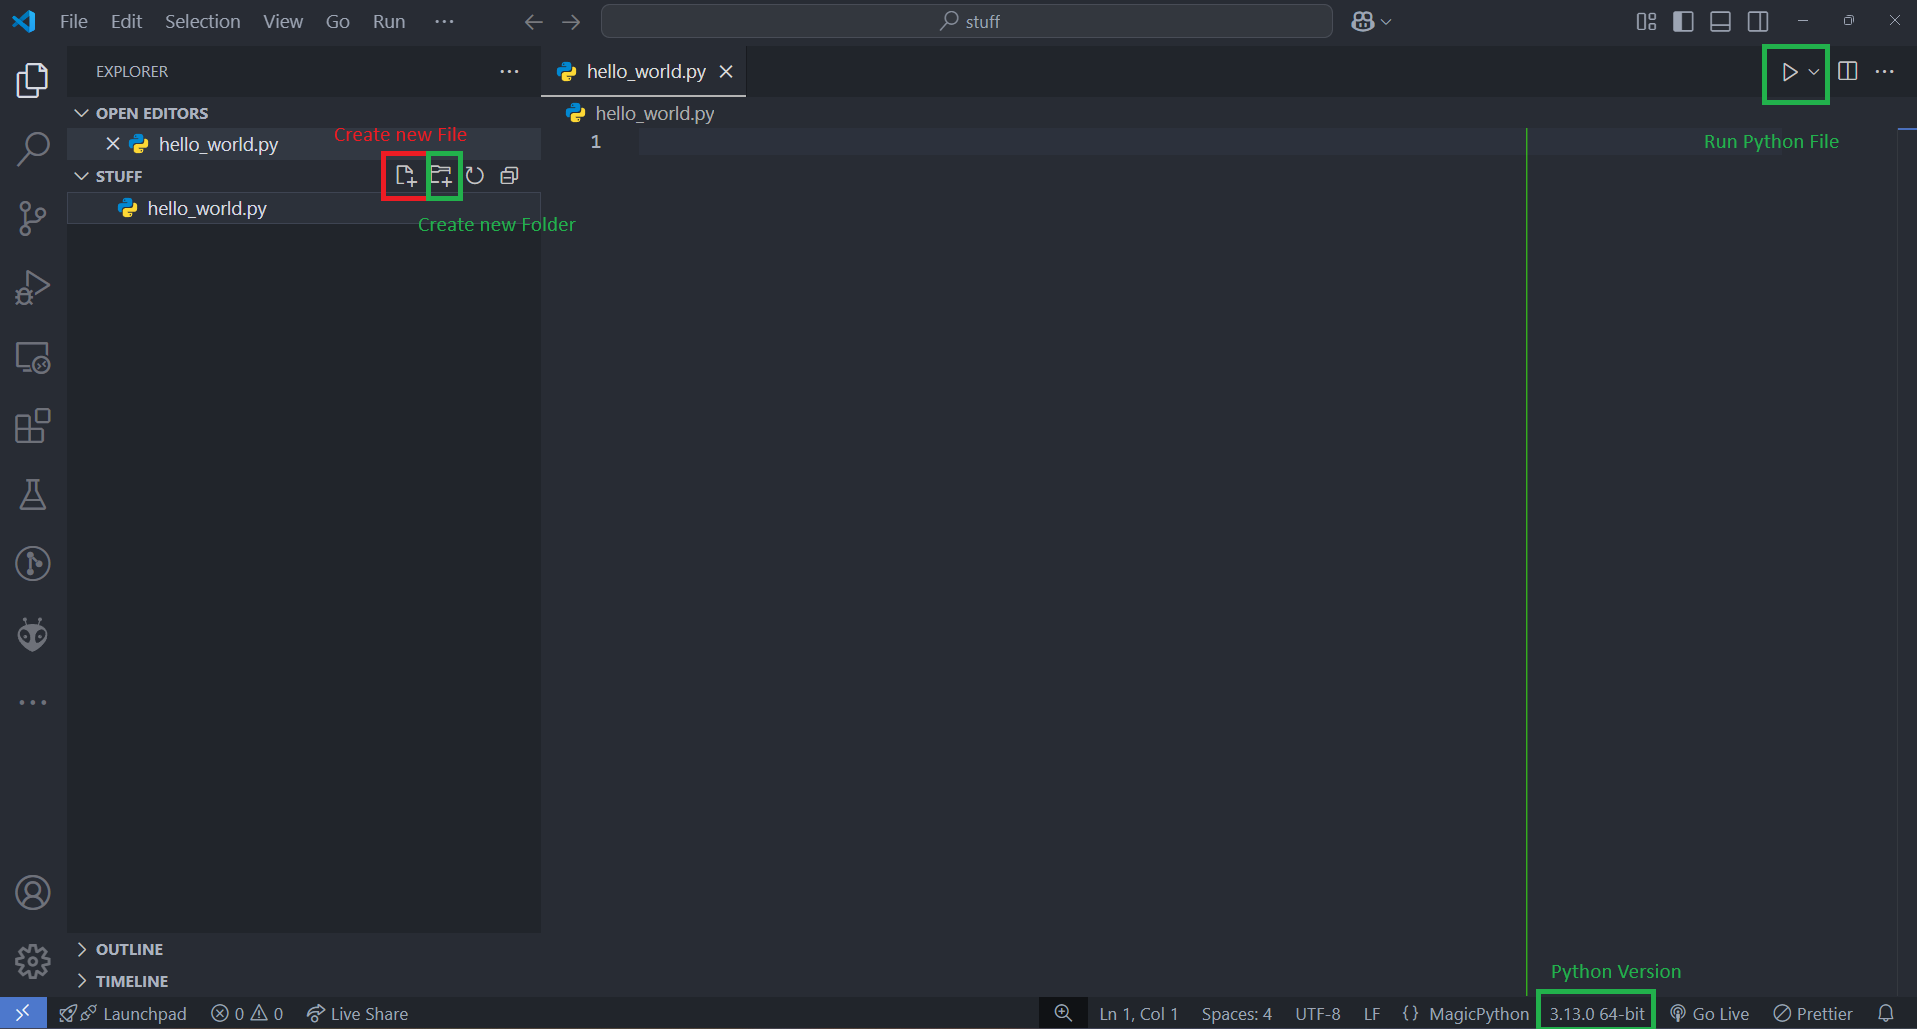
\includegraphics[width=\textwidth]{fig/VS_Code_overview.png}
  \end{center}
\end{frame}

\begin{frame}
  \frametitle{Hello World!}
  \lstinputlisting[language=python, lastline=4]{examples/hello_world.py}
  After we have written the code we click on the run button in the top right corner.\\
  We get the following output in the terminal:\\
  \vspace{5mm}
  \hspace*{-1cm} 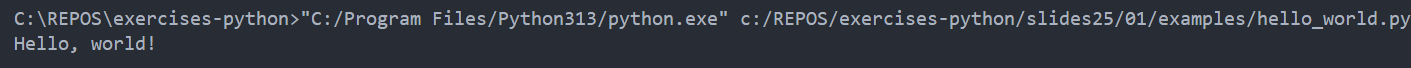
\includegraphics[width=1.16\textwidth]{fig/Hello_world_out.png}
\end{frame}
\begin{frame}[fragile]
  \frametitle{Variables: Math vs. Programming}

  \textbf{Mathematics:}  
  \begin{center}
    \large\( x = 5 \Rightarrow x \) always stays 5
  \end{center}

  \vspace{5mm}
  
  \textbf{Programming:}  
  \begin{lstlisting}[language=Python]
x = 5
x = x + 1
print(x)  # Output: 6
\end{lstlisting}
\begin{center}
  \textcolor{red}{\large\( x = 5 \Rightarrow\) value of  $x$ can be changed}
\end{center}
\end{frame}

\begin{frame}
  \frametitle{Defining variables}
  \lstinputlisting[language=python, firstline=6, lastline=10]{examples/hello_world.py}
  \vspace{5mm}
  And we can also print the variables to the terminal.\\
  \vspace{5mm}
  \lstinputlisting[language=python, firstline=13, lastline=16]{examples/hello_world.py}
\end{frame}

\begin{frame}
  \frametitle{Python as a calculator}
  \lstinputlisting[language=python, firstline=18]{examples/hello_world.py}
\end{frame}



\section{Additional Resources}
\begin{frame}
  \frametitle{Additional Resources}
  \begin{itemize}
    \item \hrefu{https://www.codewars.com/}{Codewars}
    \item \hrefu{https://leetcode.com/}{Leetcode}
    \item \hrefu{https://ohmygit.org/}{Oh my git!}
    \item \hrefu{https://www.learnpython.org/}{Interactive python tutorials}
    \item \hrefu{https://www.codecademy.com/learn/learn-python-3}{Learn Python 3}
    \item \hrefu{https://pll.harvard.edu/course/cs50-introduction-computer-science?delta=0}{CS50}
  \end{itemize}
   

\end{frame}

%%%%%%%%%%%%%%%%%%%%%%%%%%%%%%%%%%%%%%%%%%%%%%%%%%%%%%%%%%%%%%%%%%%%%%%%%%%%

\end{document}
%%%%%%%%%%%%%%%%%%%%%%%%%%%%%%%%%%%%%%%%%%%%%%%%%%%%%%%%%%%%%%%%%%%%%%%%%%%%

%% EOF

